\documentclass[12pt]{article}
% A good sample LaTeX file that you can modify and use as a template.

\usepackage{graphicx}		% Enable graphics commands
\usepackage{lscape}		% Enable landscape with \begin{landscape} until \end{landscape}
\usepackage{natbib}			% Enable citation commands \citep{}, \citet{}, etc.
\bibpunct{(}{)}{;}{a}{}{,}		% Formatting for in-text citations
\usepackage{setspace}		% Enable double-spacing with \begin{spacing}{2} until \end{spacing}.
\usepackage[utf8]{inputenc} 	% Enable utf8 characters, i.e., accents without coding--just type them in.
\usepackage[english]{babel}	% English hyphenation and alphabetization.  Other languages available.
\usepackage{dcolumn}        % For decimal-aligned stargazer output.
\usepackage[colorlinks=true, urlcolor=blue, citecolor=black, linkcolor=black]{hyperref} % Include hyperlinks with the \url and \href commands.
\setlength{\tabcolsep}{1pt}	% Make tables slightly narrower by reducing space between columns.

\renewcommand\floatpagefraction{.9}	% These commands allow larger tables and graphics to fit
\renewcommand\topfraction{.9}		% on a page when default settings would complain.
\renewcommand\bottomfraction{.9}
\renewcommand\textfraction{.1}
\setcounter{totalnumber}{50}
\setcounter{topnumber}{50}
\setcounter{bottomnumber}{50}

\newcommand{\R}{\textsf{R}~}        %This creates the command \R to typeset the name R correctly.

%\usepackage[left=1in, right=1in]{geometry}	%Turn footnotes into endnotes (commented out).
%\renewcommand{\footnotesize}{\normalsize}	
%\usepackage{endnotes}
%\renewcommand{\footnote}{\endnote}
%\renewcommand{\section}{\subsection}

\usepackage{Sweave}
\begin{document}
\Sconcordance{concordance:LaTeX_Example.tex:LaTeX_Example.Rnw:%
1 30 1 1 0 46 1 1 22 1 2 20 0 2 2 45 0 1 2 5 1 1 4 23 1}



\title{Title of Your Paper}		% Better titles available.
\author{Your Name}			% Likewise.
\date{\today}				% Replace \today with an actual date if you don't want it to change.
\maketitle

\begin{abstract}
This should be 100 to 150 words summarizing your paper.
\end{abstract}

\newpage					% Start your actual text on a clean slate.

\section{Citations}
There are many different citation packages, but I prefer the natbib package called above.  To make a parenthetical citation, you use \verb+\citep{citekey}+ (the p is for parenthetical).  To make a textual citation, you use \verb+\citet{citekey}+ (t for textual).  Put page numbers in a leading set of brackets: \verb+\citep[25-26]{citekey}+.  Put textual comments in \emph{another} set of leading brackets: \verb+\citep[see][10]{citekey}+.  Try out \verb+\citeauthor+ and \verb+\citealt+ and see what you get.  I consistently use \verb+FirstauthorYear+ for my citekeys; it's best to choose a format and stick to it so that you don't actually have to look up citekeys.  Some BibTeX software (e.g., BibDesk) will even automatically generate citekeys using the format you specify.  Okay, an example: \\

Linear regression is easy \citep[see, e.g.,][]{Gelman2007}.  But, as \citet[86-87]{Solt2001} points out, it isn't always the most appropriate technique.

\section{Tables By Hand in \LaTeX}
Doing tables by hand can get very complicated.  The key line is the one that starts \verb+\begin{tabular}+.  The next set of curly brackets define how many columns there will be and the characteristics of those columns.  The letters l, r, and c mean the column should be left-justified, right-justified, or centered, respectively.  The letter p means a column should be a paragraph with a fixed width specified by the length inside the curly brackets.  Here I've used \verb+p{.5cm}+ to get some extra space between columns.  Once you're inside the table, the \verb+&+ means ``this column is done, go on to the next one."  As you can see, the \verb+\multicolumn+ command is used to span multiple columns, for example, for a heading.  Here, I ended up inserting some spaces using \verb+\,+ to make the columns an even width, although it would have been cleaner to use p-columns.

\begin{table}[hbtp] 
\caption{Economic Inequality, Average Incomes, and Poverty in Four Hypothetical Countries}
\label{T:sim}
\begin{small}
\begin{tabular}{l p{.5cm} c c c c c c c c c c p{.5cm} c p{.5cm} c p{.5cm} c}
\\
\hline
&& \multicolumn{10}{c}{Income Decile} & & Gini & & GDP/ & & Poverty\\
\cline{3-12} Country && 1 & 2 & 3 & 4 & 5 & 6 & 7 & 8 & 9 & 10 & & Index & & Capita & & Gap\\
\hline
\\
 A && \,40\,\, & \,45\,\, & \,60\,\, & \,70\,\, & \,80\,\, & \,85\,\, & 100\, & 125\, & 145\, & 250\, && 30.1 && 100 & & 15\\
 B && \,40\,\, & \,45\,\, & \,60\,\, & \,60\,\, & \,60\,\, & \,65\,\, & 100\, & 125\, & 150\, & 300\, && 35.1 && 100 & & 15\\
 C && \,40\,\, & \,45\,\, & \,70\,\, & \,80\,\, & \,90\,\, & \,100\,\, & 105\, & 140\, & 160\, & 270\, && 30.1 && 110 & & 15\\
 D && \,40\,\, & \,45\,\, & \,45\,\, & \,85\,\, & \,85\,\, & \,85\,\, & 100\, & 120\, & 145\, & 250\, && 30.1 && 100 & & 20\\
\hline
\end{tabular}
\end{small}
\end{table}

\newpage
\section{The Stargazer Package}
Although hand-building tables is possible, it is way better to have \R generate the table you want.  As usual, there are several ways to go, but the stargazer package is a handy one (and it was written by a political scientist, so it is more likely than others to correspond to our disciplinary norms).  It has many, many options: check out \href{http://cran.r-project.org/web/packages/stargazer/stargazer.pdf}{the manual} and \href{http://cran.r-project.org/web/packages/stargazer/vignettes/stargazer.pdf}{the vignettes}.


% Table created by stargazer v.4.5.3 by Marek Hlavac, Harvard University. E-mail: hlavac at fas.harvard.edu
% Date and time: Sun, Mar 23, 2014 - 1:45:36 PM
\begin{table}[!htbp] \centering 
  \caption{Summary Statistics, State Dataset} 
  \label{T:sum} 
\begin{tabular}{@{\extracolsep{5pt}}lccccc} 
\\[-1.8ex]\hline 
\hline \\[-1.8ex] 
Statistic & \multicolumn{1}{c}{N} & \multicolumn{1}{c}{Mean} & \multicolumn{1}{c}{St. Dev.} & \multicolumn{1}{c}{Min} & \multicolumn{1}{c}{Max} \\ 
\hline \\[-1.8ex] 
alpha & 50 & 25.500 & 14.577 & 1 & 50 \\ 
regdays & 50 & 21.040 & 11.258 & 0 & 30 \\ 
stategini & 50 & 44.614 & 2.134 & 40.200 & 49.900 \\ 
stdiversity & 50 & 36.533 & 16.420 & 6.800 & 73.465 \\ 
over64 & 50 & 16.108 & 2.892 & 5.360 & 21.450 \\ 
college & 50 & 16.085 & 3.079 & 10.650 & 23.702 \\ 
stincpc & 50 & 20,767.380 & 2,848.744 & 15,853 & 28,766 \\ 
south & 50 & 0.220 & 0.418 & 0 & 1 \\ 
\hline \\[-1.8ex] 
\normalsize 
\end{tabular} 
\end{table} 
% Table created by stargazer v.4.5.3 by Marek Hlavac, Harvard University. E-mail: hlavac at fas.harvard.edu
% Date and time: Sun, Mar 23, 2014 - 1:45:36 PM
% Requires LaTeX packages: dcolumn 
\begin{table}[!htbp] \centering 
  \caption{Linear Regression Results} 
  \label{T:res} 
\begin{tabular}{@{\extracolsep{5pt}}lD{.}{.}{-3} D{.}{.}{-3} } 
\\[-1.8ex]\hline 
\hline \\[-1.8ex] 
 & \multicolumn{2}{c}{\textit{Dependent variable:}} \\ 
\cline{2-3} 
\\[-1.8ex] & \multicolumn{2}{c}{Registration Days} \\ 
\\[-1.8ex] & \multicolumn{1}{c}{(1)} & \multicolumn{1}{c}{(2)}\\ 
\hline \\[-1.8ex] 
 stategini & 1.408^{**} & 5.875^{***} \\ 
  & (0.698) & (1.479) \\ 
  & & \\ 
 stdiversity & 0.323^{***} & 5.371^{***} \\ 
  & (0.093) & (1.515) \\ 
  & & \\ 
 over64 & 0.144 & 0.178 \\ 
  & (0.438) & (0.394) \\ 
  & & \\ 
 college & -1.548^{**} & -0.916 \\ 
  & (0.760) & (0.709) \\ 
  & & \\ 
 stincpc & 0.001 & 0.001 \\ 
  & (0.001) & (0.001) \\ 
  & & \\ 
 south & -0.557 & 0.505 \\ 
  & (3.580) & (3.236) \\ 
  & & \\ 
 stategini:stdiversity &  & -0.114^{***} \\ 
  &  & (0.034) \\ 
  & & \\ 
 Constant & -59.203^{*} & -254.768^{***} \\ 
  & (32.634) & (65.553) \\ 
  & & \\ 
\hline \\[-1.8ex] 
Observations & \multicolumn{1}{c}{50} & \multicolumn{1}{c}{50} \\ 
R$^{2}$ & \multicolumn{1}{c}{0.503} & \multicolumn{1}{c}{0.607} \\ 
\hline 
\hline \\[-1.8ex] 
\textit{Note:}  & \multicolumn{2}{r}{$^{*}$p$<$0.1; $^{**}$p$<$0.05; $^{***}$p$<$0.01} \\ 
\normalsize 
\end{tabular} 
\end{table} 
\newpage

\section{Figures}
Although you can drop \textsf{R}-generated figures straight into your document using the \verb+fig=T+ code-chunk argument, I generally prefer to use \R to generate pdfs of my figures: the \verb+fig=T, include=F+ combination of arguments generates pdfs with auto-generated names of the format sweavefilename-figurelabel.pdf.  I then insert them with the commands below, which give you more control over where and how the figures appear and make it easier to include notes and the like.     

 
\begin{figure}[htbp] 
  \caption{State Registration Deadlines by Income Inequality}
  \label{F:scatter}
  \begin{center}
    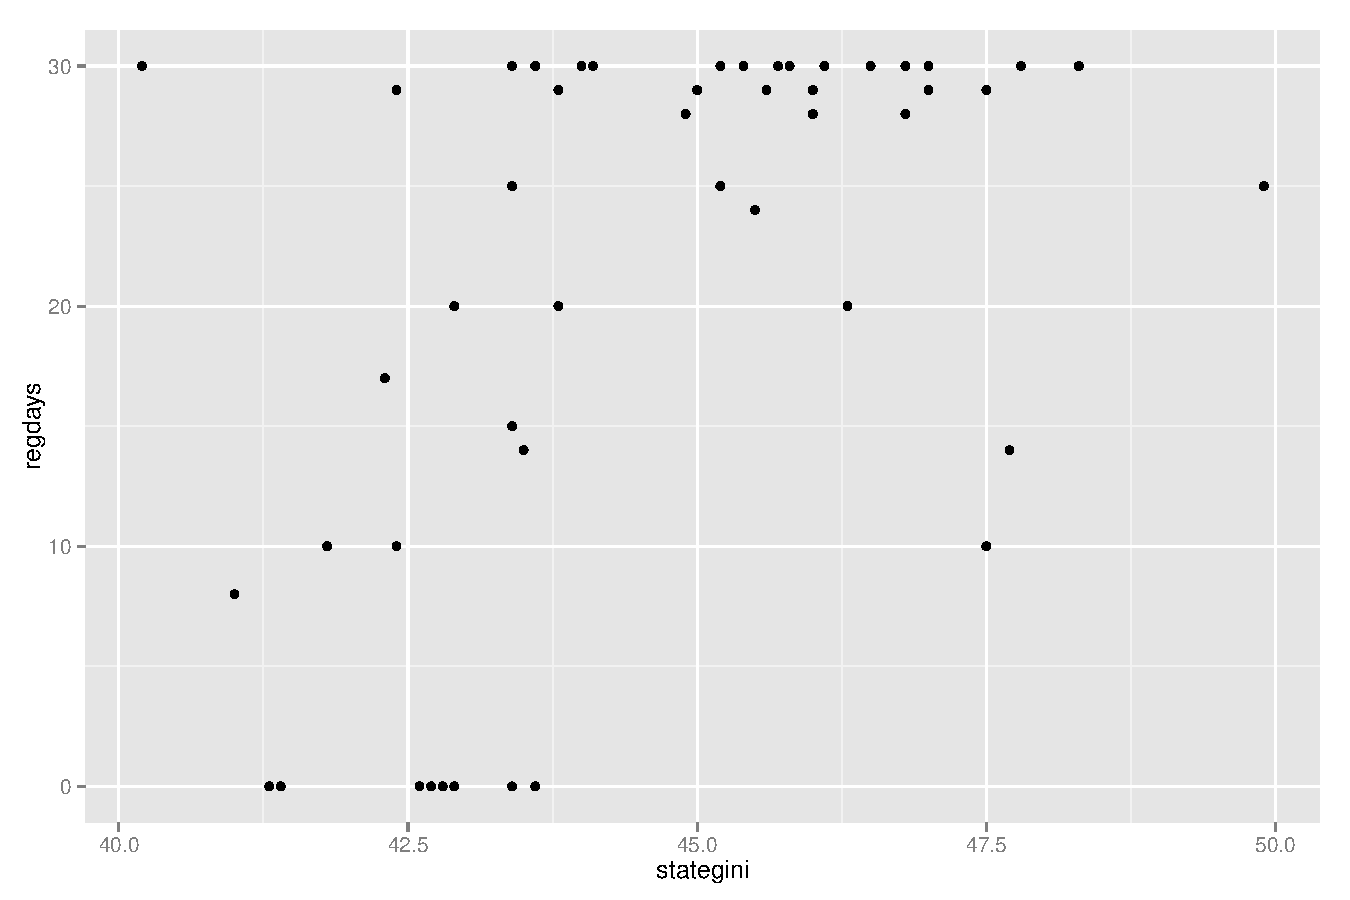
\includegraphics[width=5.25in]{LaTeX_Example-f1.pdf}
  \end{center}
  \begin{footnotesize}
  \begin{tabular}{p{.4in} p{4.75in}}
  & \emph{Note}: One should really label one's axes with descriptive names rather than just using the codenames of variables from one's dataset.  Then again, one should only include informative notes to figures rather than just making up text.
  \end{tabular}
  \end{footnotesize}
\end{figure}

Note that the \verb+\label+ command, which I use for all tables and figures, lets you refer to the table or figure by its assigned number using the \verb+\ref+ command.  You can use whatever label you want. For example, for the scatterplot in Figure~\ref{F:scatter}, I used \verb+F:scatter+.  I always put a \verb+T:+ in table labels (see my use of the \verb+label=+ option in the \verb+stargazer+ commands above) and an \verb+F:+ in figure labels, just to help keep them straight in my mind. 

\section{Bibliography}
The bibliography is easily generated using the two commands below.  The \verb+ajps+ style is one I hacked together myself based on the \verb+apsr+ style floating around the web, which neglects to put a comma after the second-to-last name in a list of three or more authors <shiver>. 

\bibliographystyle{ajps}
\bibliography{ExampleLibrary}

\end{document}

